% appendix_place.tex: the rate by place from the window profile of the within-borrower ratio (Code/local/place_windows.R;
% JH 2026-09-16: no asymmetry between score, income and geography). Numbers: results/rho_place_windows.csv, results/geo_rate_regime.csv.
\section{The Rate by Place}\label{appendix:place}

The within-borrower design of Section \ref{sec:rate_people} is run by state exactly as it is run by score decile, and the two splits behave differently in one respect. The payment elasticity by state ranges from $0.38$ to $0.74$ across the large states, as narrow a range as across deciles; the term elasticity ranges from $-0.12$ in California to $0.76$ in Indiana, three times the range across deciles, and the ratio with it. The 24-month estimate of Section \ref{sec:rate_people} rests on the condition that the balance-scaled penalty channel of Proposition \ref{prop:termmargin} has decayed by then. The condition holds pooled and, because a score decile averages over every state, decile by decile. It does not hold state by state: at twelve months every state's ratio is negative, the penalty channel dominating as it does pooled, and between twelve and twenty-four months Texas moves from $-1.20$ to $1.20$ and Georgia from $-1.30$ to $0.94$ while California moves from $-0.85$ to $-0.21$ and Arizona from $-1.29$ to $0.07$. The speed at which the penalty channel decays is a property of the place, through repossession timing and collection remedies, so one national window catches some states past the channel and others still inside it.

This appendix applies the paper's own rule place by place: each place is read at the first fixed window past its penalty channel, the smallest window at which the ratio is positive and the next window does not raise it significantly. Table \ref{tab:rho_place} reports the window profile of the ratio for the twenty largest states, the window chosen, and the rate at it, and Figure \ref{fig:rho_place_windows} shows the profiles of the twelve largest. A state whose ratio is still rising at the last available window is flagged and its rate is provisional; a state whose ratio is negative at every window has no rate; a ratio at or above the formula's ceiling gives a bound at zero. A first attempt to net the state's collection law out of the 24-month ratio as a level shift, recorded in Appendix \ref{appendix:strategies}, explains 39 percent of the cross-state variance through mortgage recourse with the sign the penalty channel does not predict and leaves 28 of 50 states outside the formula's range; a level shift is the wrong correction for a difference in timing.

The timing itself is testable against the rules that govern it. A state-by-state file of repossession and collection rules (\texttt{external/state\_repossession\_rules.csv}; every state permits self-help repossession under Article 9, so the variation is in the protections around it) records whether the state requires notice or a right to cure before repossession (15 states), whether it grants a redemption or reinstatement window after repossession (11 states, among them California, New York, Ohio, Illinois and Pennsylvania), and its wage-garnishment cap. Table \ref{tab:place_timing} regresses the swing of the ratio between the 12- and 24-month windows, and its level at each window, on these rules across the 50 states, weighted by precision. A post-repossession window lowers the swing by $0.50$ (standard error $0.15$) and the 24-month level by $0.43$ ($0.14$): where the borrower can redeem or reinstate after repossession the loss is realized later and the penalty channel is still inside the 24-month window. Pre-repossession protection raises the 12-month ratio by $0.48$ ($0.19$), the early penalty channel being smaller where repossession is delayed. The garnishment cap does nothing. Together with recourse and the deficiency bar the rules explain 30 percent of the cross-state variance of the swing and 44 percent of the 24-month level, with the signs a timing difference predicts and the level-shift attempt did not find.


\begin{table}[H]
\centering
\caption{The within-borrower ratio by state across windows, and the rate at the first window past the penalty channel}
\label{tab:rho_place}
\footnotesize
\resizebox{\textwidth}{!}{\begin{tabular}{lrrrrlrl}
\toprule
State & Loans & $R_{12}$ & $R_{24}$ & $K^*$ & Status & $\rho$ & 95\% set \\
\midrule
TX & 5,794,675 & -1.20 (0.11) & 1.20 (0.04) & 24 & past the penalty channel & 0.00 & [0.00, 0.00] \\
FL & 4,448,685 & -0.87 (0.08) & 0.46 (0.03) & 24 & past the penalty channel & 0.10 & [0.05, 0.16] \\
NY & 2,727,838 & -0.06 (0.07) & 0.36 (0.04) & 24 & past the penalty channel & 0.18 & [0.11, 0.28] \\
PA & 2,344,897 & -0.73 (0.11) & 0.40 (0.05) & 24 & past the penalty channel & 0.14 & [0.05, 0.26] \\
OH & 2,266,913 & -0.77 (0.12) & 0.75 (0.06) & 24 & past the penalty channel & 0.00 & [0.00, 0.00] \\
NC & 2,072,616 & -0.58 (0.09) & 0.86 (0.06) & 24 & past the penalty channel & 0.00 & [0.00, 0.00] \\
IL & 2,023,957 & -0.61 (0.14) & 0.63 (0.07) & 24 & past the penalty channel & 0.00 & [0.00, 0.07] \\
MI & 1,939,342 & -0.15 (0.09) & 0.54 (0.05) & 24 & past the penalty channel & 0.02 & [0.00, 0.10] \\
GA & 1,894,594 & -1.30 (0.15) & 0.94 (0.08) & 24 & past the penalty channel & 0.00 & [0.00, 0.00] \\
VA & 1,556,937 & -0.23 (0.15) & 1.00 (0.09) & 24 & past the penalty channel & 0.00 & [0.00, 0.00] \\
NJ & 1,450,438 & -0.50 (0.15) & 0.34 (0.07) & 24 & past the penalty channel & 0.21 & [0.08, 0.39] \\
IN & 1,369,787 & 0.38 (0.17) & 1.68 (0.12) & 24 & past the penalty channel & 0.00 & [0.00, 0.00] \\
AZ & 1,323,063 & -1.29 (0.17) & 0.07 (0.06) & 24 & past the penalty channel & 0.78 & [0.43, $\infty$] \\
TN & 1,312,464 & -0.21 (0.12) & 1.43 (0.11) & 24 & past the penalty channel & 0.00 & [0.00, 0.00] \\
MO & 1,230,203 & -0.62 (0.18) & 0.64 (0.11) & 24 & past the penalty channel & 0.00 & [0.00, 0.12] \\
MD & 1,082,233 & -1.39 (0.39) & 0.59 (0.12) & 24 & past the penalty channel & 0.00 & [0.00, 0.19] \\
CO & 1,028,097 & -0.68 (0.18) & 0.68 (0.10) & 24 & past the penalty channel & 0.00 & [0.00, 0.07] \\
AL & 1,014,024 & -0.90 (0.17) & 1.15 (0.11) & 24 & past the penalty channel & 0.00 & [0.00, 0.00] \\
SC & 1,011,964 & -1.56 (0.19) & 0.51 (0.09) & 24 & past the penalty channel & 0.07 & [0.00, 0.22] \\
WI & 1,005,082 & 0.14 (0.17) & 0.98 (0.12) & 24 & past the penalty channel & 0.00 & [0.00, 0.00] \\
\bottomrule
\end{tabular}
}
\vspace{0.5em}
\begin{minipage}{0.95\textwidth}
\noindent \small \textit{Notes:} The twenty largest states by loans among the 13.5 million borrowers with two or more auto loans. $R_K$ is the within-borrower term elasticity of default within $K$ months over the within-borrower payment elasticity (delta-method standard errors). $K^*$ is the first window with a positive ratio that the next window does not raise by more than $1.96$ standard errors of the difference, or the last window when the ratio is still rising there. The rate maps $R_{K^*}$ through equation \eqref{eq:window} at $K = K^*$ with the state's own marginal-utility profile and the pooled exit hazard; a ratio at or above the formula's ceiling gives zero. Windows beyond 24 months are added as the cluster stage that computes them completes.
\end{minipage}
% replication: Code/identification/I6f_within_person_by_group.R, Code/local/place_windows.R; results/identification_within_person_by_group.csv, rho_place_windows.csv
\end{table}

\begin{table}[H]
\centering
\caption{The state's repossession and collection rules and the timing of the penalty channel}
\label{tab:place_timing}
\small
\begin{tabular}{lccc}
\toprule
Regressor (specification ``all'') & R24 - R12 & R24 level & R12 level \\
\midrule
Pre-repossession notice or right to cure & $-0.195$ (0.242) & $+0.070$ (0.204) & $+0.265$ (0.227) \\
Post-repossession redemption or reinstatement & $-0.510$ (0.149) & $-0.368$ (0.126) & $+0.142$ (0.140) \\
Wage-garnishment cap (percent) & $-0.015$ (0.008) & $-0.006$ (0.007) & $+0.008$ (0.008) \\
\midrule
$R^2$, joint $p$ & 0.30, 0.0067 & 0.44, 6.8e-05 & 0.24, 0.027 \\
Post-repossession window alone & $-0.495$ (0.149) & $-0.426$ (0.144) & $+0.069$ (0.149) \\
Pre-repossession protection alone & $-0.222$ (0.217) & $+0.257$ (0.205) & $+0.479$ (0.186) \\
States & 50 & 50 & 50 \\
\bottomrule
\end{tabular}

\vspace{0.5em}
\begin{minipage}{0.95\textwidth}
\noindent \small \textit{Notes:} Precision-weighted regressions across 50 states of the within-borrower ratio's swing between the 12- and 24-month windows and of its level at each window on the state's rules: an indicator for pre-repossession notice or a statutory right to cure, an indicator for a post-repossession redemption or reinstatement window, the wage-garnishment cap in percent of disposable wages, mortgage recourse and the auto deficiency bar; standard errors in parentheses. The rules file codes each state from its statute or a legal summary with a source per state (\texttt{memos/state\_repossession\_rules\_2026-09-16.md}); rules that changed mid-sample (Arizona, California, Minnesota, New Hampshire) are coded at their current values.
\end{minipage}
% replication: Code/local/place_timing.R, Code/exhibits/make_place_timing_table.R; results/place_timing_fit.csv, external/state_repossession_rules.csv
\end{table}

\begin{figure}[H]
\centering
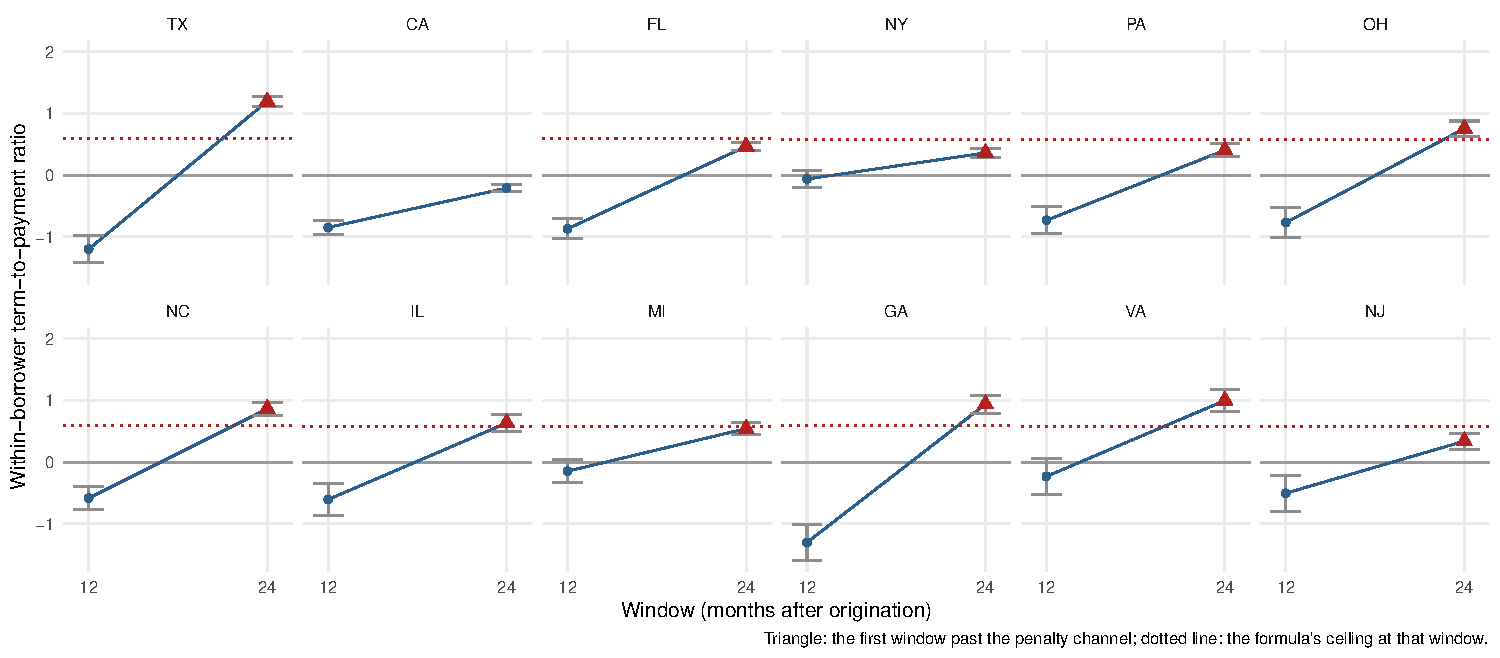
\includegraphics[width=\textwidth]{figures/fig_rho_place_windows.pdf}
\caption{The window profile of the within-borrower ratio, twelve largest states. Points and bars: the ratio at each window with 95 percent bands; the triangle marks the first window past the penalty channel and the dotted line the formula's ceiling at that window.}
\label{fig:rho_place_windows}
% replication: Code/local/place_windows.R; results/rho_place_windows.csv
\end{figure}

\subsection{The symmetric design: place by score tercile, the place fixed at the borrower's first loan}

Two constructions separate the state splits above from the score splits, and neither is a property of geography. First, a place's ratio is a ratio of averages over the place's score mix. Loan-weighted across groups the within-borrower term elasticity is $0.31$ to $0.33$ in every split, but the payment elasticity is $0.74$ within score deciles and $0.52$ within states or clusters, because a score group sorts borrowers by their default rate and a place does not; a place's ratio therefore sits where the pooled ratio sits, at the formula's ceiling, for the reason Section \ref{sec:rate_people} gives for the pooled ratio. Second, the place was the loan's, so a mover's pair was dropped, whereas score and income are the borrower's at first sight. The design of this subsection removes both: the place is the borrower's at her first loan, so both loans of every borrower fall in one place as they fall in one decile, and the within-borrower ratio is estimated in place-by-score-tercile cells (51 states and the 91 zip-code clusters, three terciles each, at 12, 24 and 36 months). A place's rate is the loan-weighted mean of its cells' rates with the decile mean's set, the headline's own construction.

Table \ref{tab:rho_place_states} and Figure \ref{fig:rho_place} report the result. Of 96 state cells with enough pairs, 34 lie inside the formula's range at 24 months; of 161 cluster cells, 61. Ten states have at least two cells inside, and their rates are on the footing of the rate by decile: Florida $0.19$ (set $0.12$ to $0.25$), New York $0.24$, Pennsylvania $0.23$, New Jersey $0.38$, Michigan $0.14$, South Carolina $0.15$, Maryland $0.11$, New Hampshire $0.09$, Colorado $0.06$ and Illinois $0.06$. Twenty-two states have every cell at or above the ceiling, among them Texas, North Carolina, Virginia, Indiana, Tennessee, Alabama, Kentucky and Louisiana, and their rates are bounds at zero; in Texas the bottom tercile's ratio is $1.29$ (standard error $0.07$) against a ceiling of $0.61$, and the cells are still rising between 24 and 36 months. The pattern is regional: the loan-weighted rate is $0.23$ across the Northeast and $0.05$ across the South and Midwest, and the share of a state's cells inside the range is higher where a post-repossession redemption or reinstatement window exists ($+0.36$, standard error $0.15$) and where income per return is higher ($+1.5$ per log point, $0.79$), with the vote and the earned-income-credit share adding nothing. Among the clusters, sixteen of 75 have two cells inside, with a median rate of $0.13$.

What the symmetric design establishes is that the excess of the term response over the preference channel across the South is not the score mix, not movers and not sampling error: it holds within borrower, within score tercile, and at three standard errors or more in the large states. The term margin in those places contains a channel that raises default with the contract's length beyond the far payments' weight, and Proposition \ref{prop:termmargin} names two candidates that a longer contract at a fixed payment moves in that direction, the balance relative to the collateral, which is the walk-away margin of Section \ref{sec:equity}, and exposure where the 36-month window does not yet remove it. Separating them needs the vehicle's value at origination, which the panel does not carry, and is the next stage; the rate by place is reported where the cells lie inside the range and as a bound elsewhere.

Across states, holding the score tercile fixed, the cell ratio is a regional object (\texttt{results/place\_cells\_correlates.csv}). Census-region effects explain 52 percent of its variance across the 129 cells with covariates; the 2020 Republican share alone explains 39 percent, $+0.28$ per standard deviation (standard error $0.03$), income per return $-0.23$, the unemployment rate $-0.22$, and mortgage recourse $+0.25$, which is a proxy for the West rather than a collection rule, since auto deficiency is permitted in every state: the 24 cells with a negative ratio at 24 months are in Alaska, Arizona, California, Connecticut, Delaware, Hawaii, Minnesota, Nevada, North Dakota, Oregon and Washington, and the cells above the ceiling are in the South. Jointly, the vote and recourse survive ($+0.12$ and $+0.18$ per standard deviation) and income does not. Within a score tercile and within borrower, then, the term response is highest where the vote is Republican and lowest on the West Coast, in both cases beyond what the preference channel allows in that direction, so the correlation is not a statement about the far payments' weight until the channel that moves the term response beyond its bound is separated from it.

\begin{table}[H]
\centering
\caption{The rate by state from place-by-score-tercile cells, twenty largest states}
\label{tab:rho_place_states}
\footnotesize
\resizebox{\textwidth}{!}{\begin{tabular}{lrrrrrr}
\toprule
State & Loans & Cells inside the range & $\rho$, cell mean & 95\% set & Pooled ratio (s.e.) & $\rho$ from the pooled ratio \\
\midrule
TX & 5,782,803 & 0 of 3 & 0.00 & [0.00, 0.01] & 1.15 (0.04) & 0.00 \\
FL & 4,418,350 & 3 of 3 & 0.19 & [0.12, 0.25] & 0.44 (0.03) & 0.12 \\
NY & 2,741,925 & 3 of 3 & 0.24 & [0.04, 0.44] & 0.36 (0.04) & 0.19 \\
PA & 2,349,869 & 3 of 3 & 0.23 & [0.02, 0.43] & 0.35 (0.05) & 0.20 \\
OH & 2,269,690 & 1 of 3 & 0.04 & [0.00, 0.12] & 0.71 (0.06) & 0.00 \\
NC & 2,066,785 & 0 of 3 & 0.00 & [0.00, 0.02] & 0.82 (0.05) & 0.00 \\
IL & 2,033,370 & 2 of 3 & 0.06 & [0.00, 0.14] & 0.60 (0.07) & 0.00 \\
GA & 1,893,724 & 1 of 3 & 0.02 & [0.00, 0.05] & 0.84 (0.07) & 0.00 \\
VA & 1,559,244 & 0 of 3 & 0.00 & [0.00, 0.06] & 0.93 (0.08) & 0.00 \\
IN & 1,371,383 & 0 of 3 & 0.00 & [0.00, 0.06] & 1.56 (0.11) & 0.00 \\
TN & 1,306,586 & 0 of 3 & 0.00 & [0.00, 0.00] & 1.46 (0.11) & 0.00 \\
MO & 1,231,035 & 1 of 3 & 0.09 & [0.00, 0.19] & 0.60 (0.10) & 0.00 \\
MI & 1,100,048 & 2 of 2 & 0.14 & [0.03, 0.24] & 0.50 (0.05) & 0.06 \\
AL & 1,011,819 & 0 of 3 & 0.00 & [0.00, 0.01] & 1.09 (0.11) & 0.00 \\
SC & 1,002,714 & 2 of 3 & 0.15 & [0.02, 0.28] & 0.48 (0.08) & 0.09 \\
OK & 831,035 & 1 of 3 & 0.01 & [0.00, 0.07] & 2.04 (0.17) & 0.00 \\
NJ & 817,880 & 2 of 2 & 0.38 & [0.08, 0.69] & 0.31 (0.07) & 0.25 \\
KY & 784,183 & 0 of 3 & 0.00 & [0.00, 0.04] & 1.22 (0.11) & 0.00 \\
MD & 732,058 & 2 of 2 & 0.11 & [0.00, 0.31] & 0.57 (0.11) & 0.01 \\
LA & 641,284 & 0 of 2 & 0.00 & [0.00, 0.04] & 1.46 (0.15) & 0.00 \\
\bottomrule
\end{tabular}
}
\vspace{0.5em}
\begin{minipage}{0.95\textwidth}
\noindent \small \textit{Notes:} The place is the state of the borrower's first auto loan. Cells are state by score tercile (the borrower's score at first sight), each estimated within borrower and origination-year cells at 24 months with at least 5,000 borrowers with two or more loans; a cell's ratio is mapped through equation \eqref{eq:window} with the cell's own marginal-utility profile and the pooled exit hazard, and a cell at or above the formula's ceiling gives zero. The state's rate is the loan-weighted mean of its cells with a delta-method set from the cells' sets, as the headline's decile mean is; ``cells inside the range'' counts cells with a ratio strictly between zero and the ceiling. The pooled ratio is the state's ratio with terciles pooled, the ratio-of-averages object, and its rate is shown beside it.
\end{minipage}
% replication: Code/identification/I6h_within_person_place_cells.R, Code/local/place_rates.R; results/identification_within_person_place_cells.csv, rho_place.csv, rho_place_cells.csv
\end{table}

\begin{figure}[H]
\centering
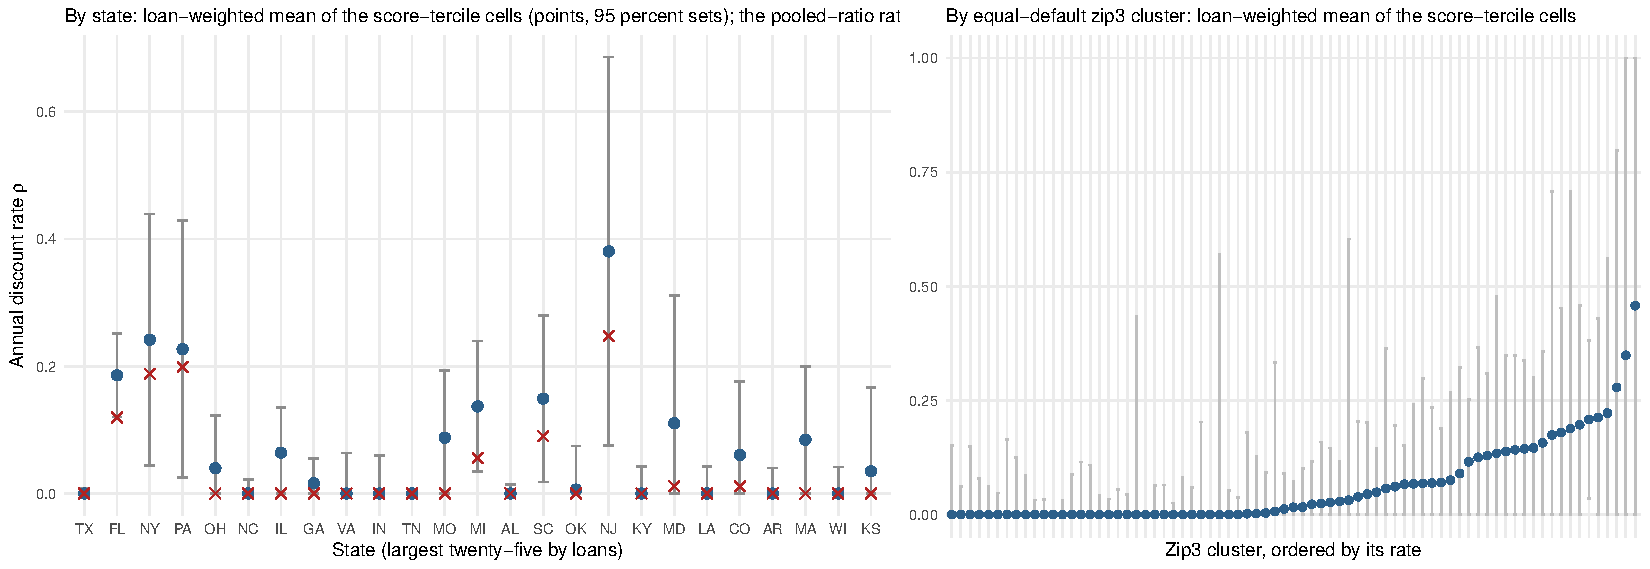
\includegraphics[width=\textwidth]{figures/fig_rho_place.pdf}
\caption{The rate by place from place-by-score-tercile cells. Left: the twenty-five largest states, the loan-weighted mean of the cells (points, 95 percent sets) and the rate from the state's pooled ratio (crosses). Right: the 91 equal-default zip-code clusters ordered by their rate. Rates and sets above one are shown at one.}
\label{fig:rho_place}
% replication: Code/local/place_rates.R; results/rho_place.csv
\end{figure}
